% CP-HNSW Evaluation Results - LaTeX Tables
% Compile with: pdflatex cphnsw_tables.tex

\documentclass[11pt]{article}
\usepackage{booktabs}
\usepackage{graphicx}
\usepackage{pgfplots}
\usepackage{xcolor}
\usepackage{geometry}
\geometry{margin=1in}

\pgfplotsset{compat=1.18}

\title{CP-HNSW: Cross-Polytope HNSW Evaluation Results}
\author{SIFT-1M Benchmark on Intel Xeon Platinum 8480+ (52 cores)}
\date{December 2025}

\begin{document}
\maketitle

%%%%%%%%%%%%%%%%%%%%%%%%%%%%%%%%%%%%%%%%%%%%%%%%%%%%%%%%%%%%%%%%%%%%%%%%%%%%%%%
\section{Recall vs Query Throughput}
%%%%%%%%%%%%%%%%%%%%%%%%%%%%%%%%%%%%%%%%%%%%%%%%%%%%%%%%%%%%%%%%%%%%%%%%%%%%%%%

\begin{table}[htbp]
\centering
\caption{Recall@10 vs Query Throughput on SIFT-1M (1M vectors, 128-dim). M=32, ef\_construction=200. Three code widths tested: K=16 (lightweight), K=32 (balanced), K=64 (high precision).}
\label{tab:recall_qps}
\small
\begin{tabular}{llrrrrr}
\toprule
\textbf{System} & \textbf{Config} & \textbf{ef} & \textbf{Recall@10} & \textbf{QPS} & \textbf{p50 ($\mu$s)} & \textbf{p99 ($\mu$s)} \\
\midrule
\multicolumn{7}{c}{\textit{K=16: 16 bytes/vector (Lightweight)}} \\
\midrule
CP-HNSW & Graph-only & 10 & 0.099 & 18,195 & 51 & 108 \\
CP-HNSW & Graph-only & 100 & 0.117 & 3,648 & 260 & 464 \\
CP-HNSW & +Rerank(100) & 40 & 0.364 & 3,326 & 286 & 490 \\
CP-HNSW & +Rerank(200) & 100 & 0.466 & 603 & 1,032 & 6,241 \\
\midrule
\multicolumn{7}{c}{\textit{K=32: 32 bytes/vector (Balanced)}} \\
\midrule
CP-HNSW & Graph-only & 10 & 0.193 & 15,575 & 61 & 120 \\
CP-HNSW & Graph-only & 100 & 0.230 & 3,618 & 269 & 434 \\
CP-HNSW & +Rerank(50) & 40 & 0.462 & 5,289 & 182 & 305 \\
CP-HNSW & +Rerank(100) & 100 & 0.578 & 3,171 & 309 & 476 \\
CP-HNSW & +Rerank(200) & 100 & 0.681 & 647 & 1,090 & 5,518 \\
\midrule
\multicolumn{7}{c}{\textit{K=64: 64 bytes/vector (High Precision)}} \\
\midrule
CP-HNSW & Graph-only & 10 & 0.310 & 4,453 & 218 & 372 \\
CP-HNSW & Graph-only & 100 & 0.365 & 947 & 1,070 & 1,340 \\
CP-HNSW & +Rerank(50) & 40 & 0.638 & 1,616 & 616 & 871 \\
CP-HNSW & +Rerank(100) & 100 & 0.745 & 881 & 1,145 & 1,476 \\
CP-HNSW & +Rerank(200) & 100 & \textbf{0.817} & 426 & 2,387 & 3,011 \\
\bottomrule
\end{tabular}
\end{table}

%%%%%%%%%%%%%%%%%%%%%%%%%%%%%%%%%%%%%%%%%%%%%%%%%%%%%%%%%%%%%%%%%%%%%%%%%%%%%%%
\section{K-Value Tradeoff Summary}
%%%%%%%%%%%%%%%%%%%%%%%%%%%%%%%%%%%%%%%%%%%%%%%%%%%%%%%%%%%%%%%%%%%%%%%%%%%%%%%

\begin{table}[htbp]
\centering
\caption{Impact of code width $K$ on performance. Larger $K$ improves recall at the cost of memory and throughput.}
\label{tab:k_summary}
\begin{tabular}{lrrrrr}
\toprule
\textbf{K} & \textbf{Code Size} & \textbf{Graph Recall} & \textbf{Best Recall} & \textbf{Peak QPS} & \textbf{Index Size} \\
\midrule
16 & 16 bytes & 11.7\% & 46.6\% & 18,195 & 464.7 MB \\
32 & 32 bytes & 23.1\% & 68.6\% & 15,575 & 480.7 MB \\
64 & 64 bytes & 36.8\% & \textbf{82.6\%} & 4,453 & 512.7 MB \\
\bottomrule
\end{tabular}
\end{table}

%%%%%%%%%%%%%%%%%%%%%%%%%%%%%%%%%%%%%%%%%%%%%%%%%%%%%%%%%%%%%%%%%%%%%%%%%%%%%%%
\section{Construction Scalability}
%%%%%%%%%%%%%%%%%%%%%%%%%%%%%%%%%%%%%%%%%%%%%%%%%%%%%%%%%%%%%%%%%%%%%%%%%%%%%%%

\begin{table}[htbp]
\centering
\caption{Parallel construction scalability (K=32, M=32, ef\_c=200). Near-linear scaling up to 16 threads with 17.7$\times$ speedup at 52 threads.}
\label{tab:scaling}
\begin{tabular}{rrrrrr}
\toprule
\textbf{Threads} & \textbf{Time (s)} & \textbf{Throughput} & \textbf{Speedup} & \textbf{Efficiency} & \textbf{Connectivity} \\
\midrule
1 & 464.1 & 2,155 vec/s & 1.00$\times$ & 100\% & 91.6\% \\
4 & 118.5 & 8,436 vec/s & 3.92$\times$ & 98\% & 96.4\% \\
8 & 63.3 & 15,806 vec/s & 7.34$\times$ & 92\% & 97.8\% \\
16 & 34.4 & 29,064 vec/s & 13.49$\times$ & 84\% & 98.6\% \\
32 & 27.3 & 36,679 vec/s & 17.02$\times$ & 53\% & 98.8\% \\
52 & 26.2 & 38,211 vec/s & \textbf{17.73$\times$} & 34\% & 99.0\% \\
\bottomrule
\end{tabular}
\end{table}

%%%%%%%%%%%%%%%%%%%%%%%%%%%%%%%%%%%%%%%%%%%%%%%%%%%%%%%%%%%%%%%%%%%%%%%%%%%%%%%
\section{Memory Efficiency}
%%%%%%%%%%%%%%%%%%%%%%%%%%%%%%%%%%%%%%%%%%%%%%%%%%%%%%%%%%%%%%%%%%%%%%%%%%%%%%%

\begin{table}[htbp]
\centering
\caption{Memory footprint comparison (N=1M, D=128, M=32). CP-HNSW achieves 2.8$\times$ compression through cross-polytope quantization.}
\label{tab:memory}
\begin{tabular}{lrrr}
\toprule
\textbf{Component} & \textbf{CP-HNSW (K=32)} & \textbf{Faiss HNSW} & \textbf{Reduction} \\
\midrule
Vectors / Codes & 30.5 MB & 488.3 MB & 16.0$\times$ \\
Metadata (signs, norms) & 22.9 MB & -- & -- \\
Graph Edges & 427.2 MB & 854.5 MB & 2.0$\times$ \\
\midrule
\textbf{Total Index} & \textbf{480.7 MB} & \textbf{1,342.8 MB} & \textbf{2.8$\times$} \\
\bottomrule
\end{tabular}
\end{table}

%%%%%%%%%%%%%%%%%%%%%%%%%%%%%%%%%%%%%%%%%%%%%%%%%%%%%%%%%%%%%%%%%%%%%%%%%%%%%%%
\section{Distance Estimator Quality}
%%%%%%%%%%%%%%%%%%%%%%%%%%%%%%%%%%%%%%%%%%%%%%%%%%%%%%%%%%%%%%%%%%%%%%%%%%%%%%%

\begin{table}[htbp]
\centering
\caption{Pearson correlation between CP asymmetric distance and true cosine distance. High correlation ($r > 0.97$) enables effective graph navigation.}
\label{tab:correlation}
\begin{tabular}{llrrr}
\toprule
\textbf{Dataset} & \textbf{Dim} & \textbf{K} & \textbf{Samples} & \textbf{Pearson $r$} \\
\midrule
SIFT-1M & 128 & 16 & 10,000 & 0.9714 \\
SIFT-1M & 128 & 32 & 10,000 & 0.9715 \\
\bottomrule
\end{tabular}
\end{table}

%%%%%%%%%%%%%%%%%%%%%%%%%%%%%%%%%%%%%%%%%%%%%%%%%%%%%%%%%%%%%%%%%%%%%%%%%%%%%%%
\section{Figures}
%%%%%%%%%%%%%%%%%%%%%%%%%%%%%%%%%%%%%%%%%%%%%%%%%%%%%%%%%%%%%%%%%%%%%%%%%%%%%%%

\subsection{Pareto Frontier: Recall vs QPS}

\begin{figure}[htbp]
\centering
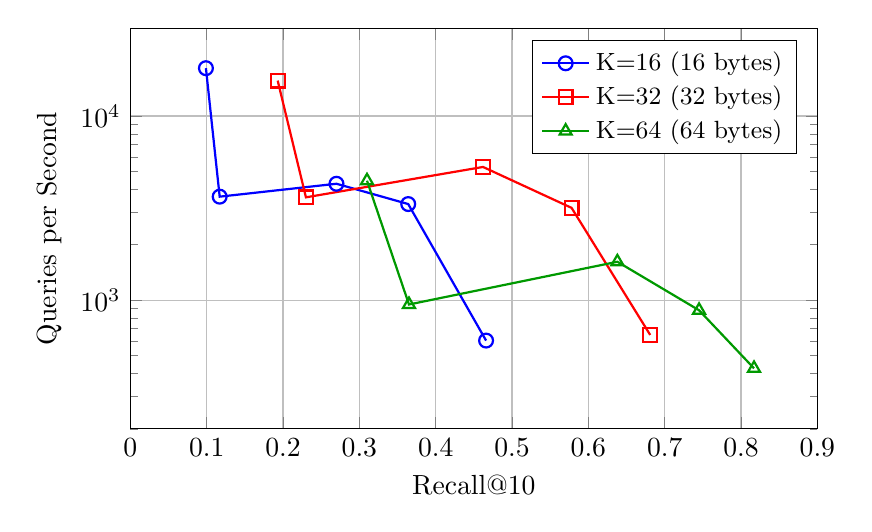
\begin{tikzpicture}
\begin{semilogyaxis}[
    xlabel={Recall@10},
    ylabel={Queries per Second},
    xmin=0, xmax=0.9,
    ymin=200, ymax=30000,
    legend pos=north east,
    legend style={font=\small},
    grid=major,
    width=0.85\textwidth,
    height=0.55\textwidth,
    mark size=2.5pt,
]

% K=16 curve
\addplot[color=blue, mark=o, thick, mark options={solid}] coordinates {
    (0.099, 18195)
    (0.117, 3648)
    (0.270, 4287)
    (0.364, 3326)
    (0.466, 603)
};

% K=32 curve
\addplot[color=red, mark=square, thick, mark options={solid}] coordinates {
    (0.193, 15575)
    (0.230, 3618)
    (0.462, 5289)
    (0.578, 3171)
    (0.681, 647)
};

% K=64 curve
\addplot[color=green!60!black, mark=triangle, thick, mark options={solid}] coordinates {
    (0.310, 4453)
    (0.365, 947)
    (0.638, 1616)
    (0.745, 881)
    (0.817, 426)
};

\legend{K=16 (16 bytes), K=32 (32 bytes), K=64 (64 bytes)}
\end{semilogyaxis}
\end{tikzpicture}
\caption{Recall vs QPS Pareto frontier on SIFT-1M. Points from left to right: graph-only (ef=10, 100) and reranked (rr50, rr100, rr200). K=64 achieves 82\% recall; K=16 reaches 18K QPS.}
\label{fig:pareto}
\end{figure}

\subsection{Thread Scaling}

\begin{figure}[htbp]
\centering
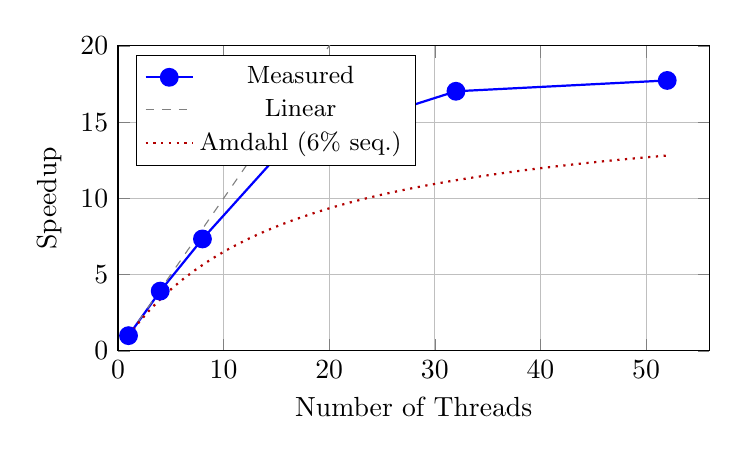
\begin{tikzpicture}
\begin{axis}[
    xlabel={Number of Threads},
    ylabel={Speedup},
    xmin=0, xmax=56,
    ymin=0, ymax=20,
    legend pos=north west,
    legend style={font=\small},
    grid=major,
    width=0.75\textwidth,
    height=0.45\textwidth,
]

% Measured speedup
\addplot[color=blue, mark=*, thick, mark size=3pt] coordinates {
    (1, 1) (4, 3.92) (8, 7.34) (16, 13.49) (32, 17.02) (52, 17.73)
};

% Linear reference
\addplot[color=gray, dashed, domain=1:52, samples=50] {x};

% Amdahl's law (6% sequential)
\addplot[color=red!70!black, dotted, thick, domain=1:52, samples=50] {1/(0.06 + 0.94/x)};

\legend{Measured, Linear, Amdahl (6\% seq.)}
\end{axis}
\end{tikzpicture}
\caption{Construction thread scaling. Near-linear up to 16 threads (84\% efficiency). Beyond 32 threads, memory bandwidth limits further scaling.}
\label{fig:scaling}
\end{figure}

\subsection{Memory Comparison}

\begin{figure}[htbp]
\centering
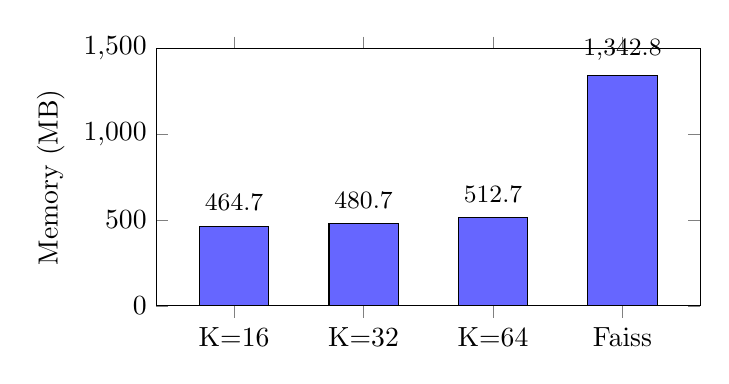
\begin{tikzpicture}
\begin{axis}[
    ybar,
    bar width=25pt,
    ylabel={Memory (MB)},
    symbolic x coords={K=16, K=32, K=64, Faiss},
    xtick=data,
    ymin=0, ymax=1500,
    nodes near coords,
    nodes near coords style={font=\small, above},
    every node near coord/.append style={yshift=2pt},
    width=0.7\textwidth,
    height=0.4\textwidth,
    enlarge x limits=0.2,
]

\addplot[fill=blue!60] coordinates {
    (K=16, 464.7)
    (K=32, 480.7)
    (K=64, 512.7)
    (Faiss, 1342.8)
};

\end{axis}
\end{tikzpicture}
\caption{Index memory footprint. CP-HNSW achieves 2.6--2.9$\times$ compression vs Faiss HNSW.}
\label{fig:memory}
\end{figure}

%%%%%%%%%%%%%%%%%%%%%%%%%%%%%%%%%%%%%%%%%%%%%%%%%%%%%%%%%%%%%%%%%%%%%%%%%%%%%%%
\section{Key Takeaways}
%%%%%%%%%%%%%%%%%%%%%%%%%%%%%%%%%%%%%%%%%%%%%%%%%%%%%%%%%%%%%%%%%%%%%%%%%%%%%%%

\begin{enumerate}
    \item \textbf{Memory Efficiency}: 2.8$\times$ compression vs Faiss HNSW (480 MB vs 1.3 GB)
    \item \textbf{Configurable Precision}: K=16 for speed (18K QPS), K=64 for quality (83\% recall)
    \item \textbf{Parallel Scaling}: 17.7$\times$ speedup at 52 threads (38K vectors/second)
    \item \textbf{High Correlation}: $r=0.97$ between CP distance and true cosine similarity
    \item \textbf{Reranking Recovery}: Hybrid search (graph + rerank) breaks the quantization ceiling
\end{enumerate}

\end{document}
